\chapter{Analiza wymagań}
% TO DO: dodać jakieś zagajenie

Analiza wymagań to kluczowy etap procesu tworzenia oprogramowania, który ma na celu zrozumienie potrzeb użytkowników oraz specyfikacji systemu. W przypadku projektowania aplikacji typu Elektroniczne Biuro Obsługi Klienta (eBOK) dla wspólnoty mieszkaniowej, istotne jest zidentyfikowanie wszystkich funkcjonalności, które będą odpowiadały zarówno mieszkańcom, jak i administratorom. Poprawna analiza wymagań pozwala na stworzenie systemu, który nie tylko spełnia potrzeby użytkowników, ale także jest skalowalny, bezpieczny i łatwy w utrzymaniu.

W niniejszym rozdziale zostaną omówione zarówno funkcjonalne, jak i niefunkcjonalne wymagania systemu, uwzględniając różnorodne potrzeby użytkowników. Przeanalizowane zostaną także kluczowe aspekty, takie jak bezpieczeństwo, wydajność, intuicyjność interfejsu, a także integracja z innymi systemami. Wymagania te będą stanowiły podstawę do zaprojektowania architektury systemu oraz jego implementacji.

\section{Zarys architektury systemu}
% TO DO: przedstawić (na diagramach poglądowych), jak ma wyglądać architektura systemu (z jakich komponentów będzie się ona składać, kto z niej będzie korzystać, jakie interfejsy będzie udostępniać). Może z tego będzie trzeba zrobić osobny rozdział.

Zarys architektury systemu jest kluczowym krokiem w projektowaniu oprogramowania, który pozwala na stworzenie efektywnego i funkcjonalnego rozwiązania. W przypadku aplikacji Elektronicznego Biura Obsługi Klienta (eBOK) dla wspólnoty mieszkaniowej, architektura musi uwzględniać zarówno potrzeby użytkowników, jak i wymagania techniczne. W tym rozdziale przedstawione zostaną główne komponenty systemu oraz ich wzajemne interakcje, na podstawie przedstawionego schematu.

\subsection{Komponenty systemu}

Architektura systemu eBOK składa się z kilku kluczowych komponentów, które współpracują ze sobą, aby zapewnić pełną funkcjonalność aplikacji. Do głównych komponentów należą:

\begin{itemize} 

	\item \textbf{Frontend} - Interfejs użytkownika aplikacji, zrealizowany w technologii Next.js, pisany w TypeScript. Frontend obsługuje interakcje użytkowników (mieszkańców oraz administratorów) oraz prezentuje dane w odpowiednim formacie. Komunikacja z backendem odbywa się za pośrednictwem bezpiecznego protokołu HTTPS, a dane są szyfrowane, przy pomocy protokołu TLS.

	\item \textbf{Backend} - Serwer aplikacji oparty na Spring Boot, działający w kontenerze Docker, odpowiedzialny za logikę biznesową oraz zarządzanie danymi. Backend zapewnia funkcje takie jak autoryzacja użytkowników (przez OAuth 2.0), obsługa zgłoszeń mieszkańców, zarządzanie płatnościami i komunikacja z zewnętrznymi systemami.

	\item \textbf{Warstwa logiki biznesowej} - Kluczowa część backendu odpowiedzialna za implementację reguł biznesowych, które obsługują funkcjonalności aplikacji, takie jak przetwarzanie zgłoszeń czy zarządzanie danymi użytkowników.

	\item \textbf{Warstwa dostępu do danych} - Odpowiada za komunikację z bazą danych PostgreSQL, przechowującą informacje dotyczące użytkowników, zgłoszeń, płatności i innych istotnych danych. Ta warstwa zapewnia trwałość i integralność danych w systemie.

	\item \textbf{Baza danych} - System PostgreSQL, działający w kontenerze Docker, przechowujący wszystkie kluczowe dane aplikacji. Dzięki konteneryzacji możliwe jest łatwe skalowanie i zarządzanie bazą danych w środowisku produkcyjnym.

	\item \textbf{Serwer OAuth 2.0} - Serwer autoryzacji, który zapewnia bezpieczeństwo dostępu do zasobów systemu przez użytkowników. OAuth 2.0 umożliwia zarządzanie autoryzacją dostępu, co zwiększa bezpieczeństwo aplikacji.

	\item \textbf{Systemy zewnętrzne} - Aplikacja integruje się z zewnętrznymi systemami, takimi jak bankowość (np. obsługa płatności online) oraz urządzenia zewnętrzne (np. liczniki zużycia mediów), co umożliwia kompleksową obsługę mieszkańców i automatyzację procesów.

\end{itemize}

\subsection{Interakcje między komponentami}

Interakcje między komponentami są kluczowe dla sprawnego funkcjonowania systemu. W architekturze tej wykorzystano konteneryzację przy pomocy Dockera, co umożliwia izolowanie poszczególnych elementów systemu oraz ułatwia to skalowanie.

\begin{itemize} 
	\item \textbf{Frontend i Backend} - Frontend wysyła zapytania HTTPS do backendu, poprzez zabezpieczenie protokołem TLS, w celu pobrania lub wysłania w sposób bezpieczny danych. Backend przetwarza te zapytania, wykonuje odpowiednie operacje na bazie danych i zwraca odpowiedzi do frontendu. Dane są wysyłane i odbierane w formacie JSON.
	
	\item \textbf{Backend i Baza danych} - Backend łączy się z bazą danych PostgreSQL w celu odczytu i zapisu danych. Wszystkie operacje na danych, takie jak dodawanie nowych zgłoszeń czy aktualizacja informacji o płatnościach, są realizowane przez backend.

	\item \textbf{Backend i System płatności} - Backend integruje się z systemami płatności, aby obsługiwać transakcje finansowe. Po dokonaniu płatności, system płatności przekazuje informacje zwrotne do backendu, który aktualizuje status płatności w bazie danych.

	\item \textbf{Backend i System powiadomień} - Backend wysyła powiadomienia do systemu powiadomień w celu informowania użytkowników o ważnych zdarzeniach. System powiadomień następnie dostarcza te informacje do użytkowników za pomocą e-maili lub SMS-ów.

\end{itemize}

\subsection{Diagramy architektury}

Aby wizualizować złożoność architektury systemu eBOK, można posłużyć się diagramami. Poniżej przedstawione są przykłady diagramów, które ilustrują strukturę i interakcje poszczególnych komponentów:

\begin{figure}[H]
	\centering
		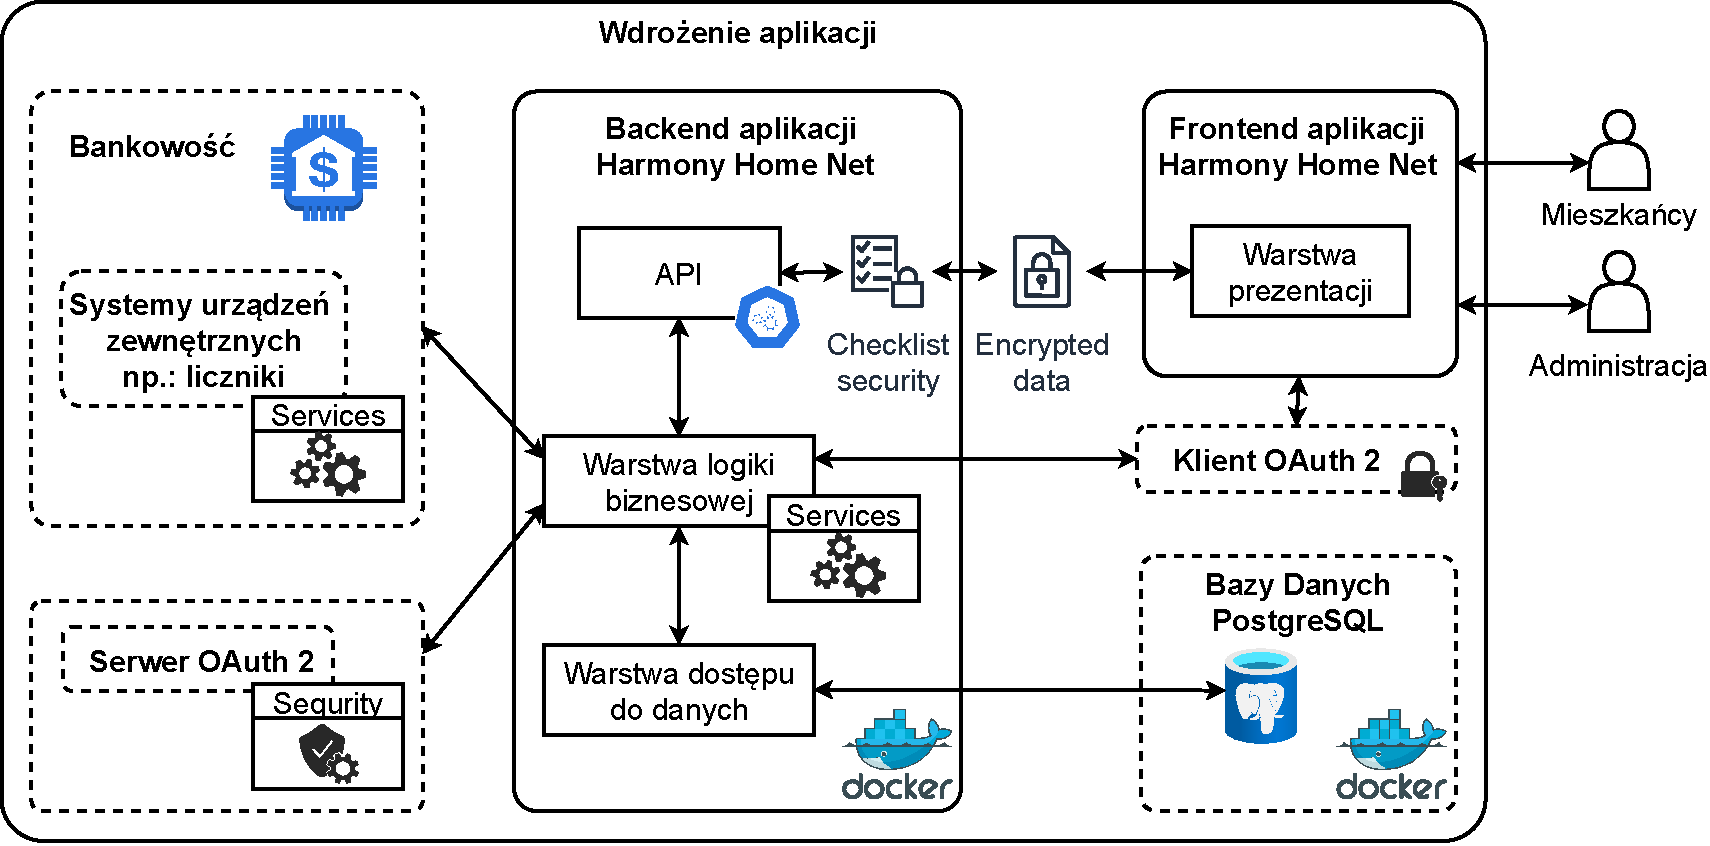
\includegraphics[width=1.1\linewidth]{Schematy/zarys_architektury}
		\caption{Schemat przestawiający zarys architektury systemu}
	\label{fig:zarys_architektury}
\end{figure}



\section{Wymagania aplikacji}
% TO DO: chyba na początek warto wyróżnić, w jakich rolach występować będą użytkownicy systemu i w ogóle - do czego ma służyć tworzona aplikacja

% Proszę zastanowić się, czy jednak nie dałoby się poniższego opisu jakoś rozwinąć (żeby nie był jedynie listą wyliczeniową). Czytelnik powinien zrozumieć, po co i dlaczego zdefiniowano poniższe wymagania. 

% Proszę zwrócić uwagę na "grupowanie" wymagań. Napisał Pan "Administrator zarządza lokalami ..." - ale trudno znaleźć wyjaśnienie, czym są te lokale i w ogóle - jaki to przypadek użycia (jaki jest kontekst, w jakim działać ma aplikacja).

Tworzona aplikacja eBOK jest narzędziem umożliwiającym efektywne zarządzanie wspólnotami mieszkaniowymi, zarówno z perspektywy mieszkańców, jak i administracji. Współczesne wspólnoty borykają się z wieloma wyzwaniami, które związane są z utrzymaniem transparentnej komunikacji między mieszkańcami a zarządcami, jak również z zapewnieniem sprawnej obsługi technicznej budynków, płatności oraz dokumentów. W związku z tym zdefiniowane wymagania aplikacji mają na celu zapewnienie takich funkcji, które sprostają tym wyzwaniom, ułatwiając codzienną administrację wspólnotą i minimalizując potrzebę fizycznych interakcji.

\subsection{Przykłady użycia aplikacji}

Aplikacja eBOK ma kilka głównych przypadków użycia, które ilustrują sytuacje, w jakich różni użytkownicy będą korzystać z jej funkcji. Na przykład, mieszkaniec może zalogować się do aplikacji, aby sprawdzić swoje należności za bieżące rachunki i zapłacić online. Jeżeli zauważy usterkę w swoim mieszkaniu (np. przeciek lub pęknięcia na ścianie), może natychmiastowo zgłosić to przez aplikację, dołączając zdjęcia, a następnie śledzić status zgłoszenia. Z kolei administrator może delegować zgłoszenie do odpowiedniego wykonawcy i monitorować proces naprawy.
Różni użytkownicy mają różne potrzeby, stąd aplikacja obsługuje dwie główne grupy użytkowników:

\begin{itemize} 

	\item \textbf{Mieszkańcy:} właściciele i najemcy, którzy korzystają z aplikacji do zarządzania swoimi płatnościami, zgłaszania usterek oraz dostępu do dokumentów. 
	
	\item \textbf{Administratorzy:} osoby zarządzające wspólnotą, odpowiedzialne za obsługę zgłoszeń, zarządzanie lokalami i mieszkańcami oraz organizację głosowań.
	
\end{itemize}

Każda z tych grup użytkowników ma dostęp do odpowiednich funkcji aplikacji, które spełniają jej potrzeby.

\subsection{Wymagania funkcjonalne}

Wymagania funkcjonalne aplikacji eBOK zostały podzielone na główne obszary tematyczne, które odpowiadają kluczowym funkcjom systemu.

\begin{enumerate}[label=\arabic*.] 

	\item \textbf{Zarządzanie kontem użytkownika:} Użytkownicy muszą mieć możliwość zakładania konta i zarządzania swoimi danymi osobowymi. Na przykład, mieszkaniec może zalogować się do systemu, aby zmienić swoje dane kontaktowe, przypisać lokal do swojego konta, a także nadawać uprawnienia członkom rodziny lub najemcom. Tego rodzaju funkcje są kluczowe dla zapewnienia personalizacji i dostępu do odpowiednich zasobów.
	
	\item \textbf{Przegląd i płatność należności:} System musi umożliwiać mieszkańcom łatwy dostęp do informacji o swoich należnościach i płatnościach. Każdy mieszkaniec powinien móc przeglądać historię swoich rachunków oraz opłacać je bezpośrednio online. Powiadomienia o zaległych płatnościach pomagają mieszkańcom pamiętać o terminach, co zmniejsza ryzyko opóźnień.

	\item \textbf{Obsługa zgłoszeń:} W przypadku usterek technicznych, takich jak wycieki czy problemy z ogrzewaniem, mieszkańcy mogą zgłaszać problemy za pośrednictwem aplikacji. Zgłoszenia te są następnie przydzielane przez administratora do odpowiednich wykonawców, a użytkownicy mogą śledzić postęp prac, co zapewnia pełną transparentność i szybką reakcję na problemy.

	\item \textbf{Zarządzanie dokumentami:} Aplikacja pełni funkcję cyfrowego archiwum dokumentów związanych ze wspólnotą, takich jak umowy, regulaminy i faktury. Mieszkańcy mogą przeglądać i pobierać dokumenty, co eliminuje potrzebę fizycznych archiwów i ułatwia dostęp do ważnych informacji.

	\item \textbf{Zarządzanie głosowaniami:} Wspólnoty mieszkaniowe często muszą podejmować ważne decyzje dotyczące administracji budynkiem lub finansów. Aplikacja umożliwia organizację i monitorowanie głosowań w formie elektronicznej, co przyspiesza podejmowanie decyzji i angażuje większą liczbę mieszkańców.

	\item \textbf{Powiadomienia:} Powiadomienia o ważnych wydarzeniach, takich jak nadchodzące głosowania, zmiany w regulaminach lub status zgłoszeń technicznych, zapewniają mieszkańcom bieżące informacje bez konieczności częstego logowania się do aplikacji. Możliwość personalizacji powiadomień zapewnia lepsze dostosowanie aplikacji do indywidualnych potrzeb użytkowników.

	\item \textbf{Panel administracyjny:} Administratorzy zarządzają całym systemem poprzez intuicyjny panel, który umożliwia im monitorowanie zgłoszeń, generowanie raportów finansowych i technicznych oraz zarządzanie kontami mieszkańców. Tego typu funkcjonalność jest kluczowa dla sprawnego zarządzania wspólnotą.

	\item \textbf{Interakcje z zewnętrznymi systemami:} Aplikacja musi umożliwiać integrację z innymi systemami, takimi jak systemy liczników mediów czy systemy płatności. Taka integracja zapewnia automatyzację wielu procesów, co redukuje błędy i obciążenia administracyjne.

\end{enumerate}

\subsection{Wymagania niefunkcjonalne}

\begin{enumerate}[label=\arabic*.] 

	\item \textbf{Skalowalność:} System musi być skalowalny, aby mógł obsługiwać zarówno małe wspólnoty, jak i duże spółdzielnie. Dzięki możliwości dynamicznego przydzielania zasobów serwerowych, system będzie w stanie dostosować się do rosnącej liczby użytkowników bez obniżenia wydajności.
	
	\item \textbf{Dostępność:} Aplikacja musi być dostępna przez całą dobę i z każdego urządzenia posiadającego dostęp do Internetu, co umożliwia użytkownikom zarządzanie swoimi sprawami w dogodnym dla nich momencie.

	\item \textbf{Bezpieczeństwo:} Wymagane są zaawansowane mechanizmy bezpieczeństwa, takie jak szyfrowanie danych, uwierzytelnianie dwuskładnikowe oraz zabezpieczenia przed atakami typu SQL Injection czy XSS. Bezpieczeństwo danych mieszkańców i transakcji jest priorytetem.

	\item \textbf{Wydajność:} System musi działać szybko i niezawodnie, nawet podczas dużego obciążenia, co ma kluczowe znaczenie dla użytkowników. Wydajność aplikacji będzie mierzona na podstawie szybkości odpowiedzi systemu oraz czasów ładowania kluczowych funkcji, takich jak zgłoszenia czy płatności.

	\item \textbf{Intuicyjność interfejsu:} Aplikacja musi być łatwa w obsłudze, z prostym i przejrzystym interfejsem dostosowanym do różnych typów użytkowników. Personalizowane pulpity dostosowują widok do potrzeb użytkownika, co zwiększa efektywność korzystania z systemu.
	
\end{enumerate}
